%% LaTeX-Beamer template for KIT design
%% by Erik Burger, Christian Hammer
%% title picture by Klaus Krogmann
%%
%% version 2.1
%%
%% mostly compatible to KIT corporate design v2.0
%% http://intranet.kit.edu/gestaltungsrichtlinien.php
%%
%% Problems, bugs and comments to
%% burger@kit.edu

\documentclass[18pt]{beamer}

%% SLIDE FORMAT

% use 'beamerthemekit' for standard 4:3 ratio
% for widescreen slides (16:9), use 'beamerthemekitwide'

\usepackage{templates/beamerthemekit}
% \usepackage{templates/beamerthemekitwide}

\usepackage[utf8]{inputenc}
\usepackage{hyperref}
\usepackage{listings}

%% TITLE PICTURE

% if a custom picture is to be used on the title page, copy it into the 'logos'
% directory, in the line below, replace 'mypicture' with the
% filename (without extension) and uncomment the following line
% (picture proportions: 63 : 20 for standard, 169 : 40 for wide
% *.eps format if you use latex+dvips+ps2pdf,
% *.jpg/*.png/*.pdf if you use pdflatex)

\titleimage{greendrop}

%% TITLE LOGO

% for a custom logo on the front page, copy your file into the 'logos'
% directory, insert the filename in the line below and uncomment it

%\titlelogo{mylogo}

% (*.eps format if you use latex+dvips+ps2pdf,
% *.jpg/*.png/*.pdf if you use pdflatex)

%% TikZ INTEGRATION

% use these packages for PCM symbols and UML classes
% \usepackage{templates/tikzkit}
% \usepackage{templates/tikzuml}

% the presentation starts here

\title[Einführung in Objektorientierte Programmierung]{Programmieren:\\ Einführung in Objektorientierte Programmierung}
\subtitle{Tutorium 30}
\author{YouniS Bensalah}
\date{November 6, 2015}

\institute{Chair for Software Design and Quality}

% Bibliography

\usepackage[citestyle=authoryear,bibstyle=numeric,hyperref,backend=biber]{biblatex}
\addbibresource{templates/example.bib}
\bibhang1em

\begin{document}

% change the following line to "ngerman" for German style date and logos
\selectlanguage{english}

%title page
\begin{frame}
\titlepage
\end{frame}

%table of contents
\begin{frame}{Heute}
\tableofcontents
\end{frame}

\section{Organisatorisches}

\begin{frame}{Freie Termine in Do-Tutorien}
    Es gibt noch freie Plätze (ca. 14) in folgenden Tutorien:
    \begin{itemize}
        \item Do 11:30 - 13:00, 50.34 Raum -120 (Peter Oettig)
        \item Do 11:30 - 13:00, 50.34 Raum -119 (Florian Heller)
    \end{itemize}
    Die Studenten, die ihr Tutorium wechseln möchten, können eine E-Mail an folgende Adresse schicken:\\
    \begin{center}
    {\Large programmieren-vorlesung@ipd.kit.edu}
    \end{center}
\end{frame}

\begin{frame}{Studierende ohne KIT-Account}
    \textbf{Hat jemand noch keinen KIT-Account (\texttt{uxxxx}) ?}
    \pause
    \begin{itemize}
        \item Kein ILIAS-Zugriff: Folien auf \url{http://younishd.fr/prog}
        \item \alert{Kein Praktomat-Zugriff: Deadline für Login ist \textbf{12.11.2015}}
        \item Nur wer bis dahin noch \textit{keinen} KIT-Account haben sollte, darf einmalig per E-Mail (\texttt{younis.bensalah@riseup.net}) an mich abgeben.
        \item Deadline muss \textbf{in jedem Fall} eingehalten werden !
    \end{itemize}
\end{frame}

\section{Nachtrag zu JDK}

\begin{frame}{Nachtrag zu JDK}
    \begin{itemize}
        \item JDK 8 ist auch ok
        \item \alert{Aufpassen bei \texttt{split()} in \texttt{String} bzw. \texttt{Pattern}}
        \item \url{http://stackoverflow.com/questions/22718744}
    \end{itemize}
\end{frame}

\section{Aufzählungstypen}

\begin{frame}{Aufzählungstypen}
    \begin{block}{Aufzählungstyp}
        Ein \textbf{Aufzählungstyp} (\textit{enumerated type}) ist ein Datentyp für Variablen mit einer endlichen Wertemenge.
    \end{block}

    \begin{exampleblock}{Beispiele}
        \begin{itemize}
            \item Wochentage
            \item Monate
            \item Himmelsrichtungen
            \item Grundfarben (RGB)
            \item Zustände eines endlichen Automaten
            \item \dots
        \end{itemize}
    \end{exampleblock}
\end{frame}

\begin{frame}[fragile]{enum in Java}
    In Java erstellt man einen solchen Aufzählungstyp mit \texttt{enum}.
    \begin{exampleblock}{\texttt{enum}}
        \begin{lstlisting}[language=Java]
public enum Day {
    MONDAY,
    TUESDAY,
    WEDNESDAY,
    THURSDAY,
    FRIDAY,
    SATURDAY,
    SUNDAY
}
        \end{lstlisting}
    \end{exampleblock}
\end{frame}

\begin{frame}[fragile]{enum in Java}
    \begin{exampleblock}{\texttt{enum} in Aktion}
        \begin{lstlisting}[language=Java]
public enum Day {...}

Day someday;

someday = Day.MONDAY;           // ok
someday = Day.TUESDAY;          // auch ok

someday = Day.JULY;             // fehler
someday = 42;                   // auch fehler
        \end{lstlisting}


    \end{exampleblock}

\end{frame}

\section{Objektorientierung}

\begin{frame}{Objektorientierung}
    \begin{figure}
        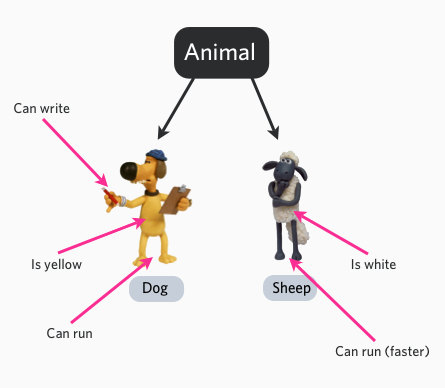
\includegraphics[scale=0.4]{img/animalclass.png}
    \end{figure}
\end{frame}

\begin{frame}{Objektorientierung}
    Worum geht es bei \textbf{Objektorientierung} ?
    \begin{itemize}
        \item Abstraktion der realen Welt
        \item Beschreibung komplexer Systeme durch das Zusammenspiel kooperierender Objekte
        \item Modellierung realer Objekte
        \item Modellieren != Programmieren
    \end{itemize}
    \textit{Hier ist noch nicht die Rede von Programmieren.}
\end{frame}

\begin{frame}{Objektorientierung}
    Was versteht man unter einem \textbf{Objekt} ?
    \begin{itemize}
        \item Alles kann ein Objekt sein !
        \item Die Frage ist vielmehr: \textit{Ist es sinnvoll ?}
        \item Ein Objekt \textit{besitzt} \textbf{Attribute} und \textit{beherrscht} \textbf{Methoden}.
        \item \textit{Welche} hängt von der Modellierung ab !
    \end{itemize}
\end{frame}

\begin{frame}{Methoden und Attribute}
    \begin{block}{Methoden}
        Methoden sind die \textbf{Aktionen}, welche ein Objekt ausführen kann.
    \end{block}

    \begin{block}{Attribute}
        Attribute sind die \textbf{Eigenschaften}, die den Zustand eines Objekts definieren.
    \end{block}
\end{frame}

\begin{frame}{Methoden und Attribute}
    \begin{exampleblock}{Methoden}
        \begin{itemize}
            \item Eine \textbf{Kaffeemaschine} kann \textbf{Kaffee kochen}.
            \item Ein \textbf{Auto} kann \textbf{fahren}.
            \item Ein \textbf{GPS} kann eine \textbf{Route berechnen}.
            \item \dots
        \end{itemize}
    \end{exampleblock}
    \begin{exampleblock}{Attribute}
        \begin{itemize}
            \item Eine \textbf{Kaffeemaschine} hat einen \textbf{Wasserstand}.
            \item Ein \textbf{Auto} hat einen aktuellen \textbf{Tachowert}.
            \item Ein \textbf{GPS} hat eine aktuelle \textbf{Position des Fahrzeugs}.
            \item \dots
        \end{itemize}
    \end{exampleblock}
\end{frame}

\begin{frame}{Beispiel: Bibliothek}
    \begin{figure}
        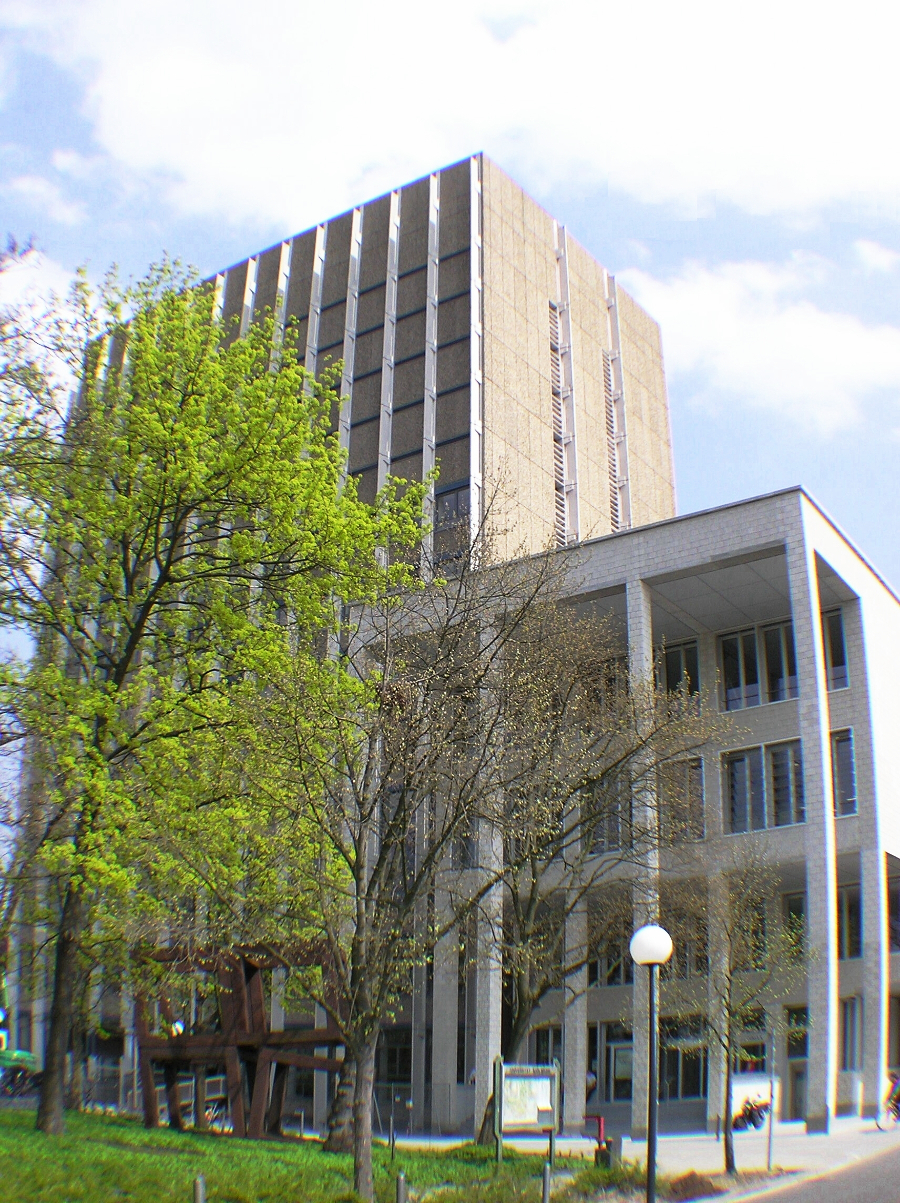
\includegraphics[scale=0.15]{img/kit_bib_sued.jpg}
    \end{figure}
\end{frame}

\begin{frame}{Bibliothek - Modellierungsversuch}
    Ziel: \textbf{Modellierung einer Bibliothek}\\
    Dabei kommen einige Fragen auf:
    \begin{itemize}
        \item Eine Bibliothek ist ein komplexes System.
        \begin{itemize}
            \item Welche Aspekte möchten wir in unserem Modell beibehalten ?
            \item Welche Details möchten wir dabei ausblenden ?
            \item Welche Informationen interessieren uns ?
            \item Wie weit dürfen wir das Modell vereinfachen ?
            \item \dots
        \end{itemize}
        \item Eine Bibliothek besteht aus kleineren Teilsystemen.
        \begin{itemize}
            \item Wie tief muss ich diese Hierarchie beibehalten ?
            \item Wie hängen diese Teilsysteme miteinander zusammen ?
            \item \dots
        \end{itemize}
    \end{itemize}
\end{frame}

\begin{frame}{Bibliothek - Modellierungsversuch}
    Problem: Wir können diese Fragen noch nicht beantworten !\\
    Vorher: \textbf{Wozu soll das Modell verwendet werden ?}
    \pause
    \begin{itemize}
        \item Erstellen eines Wegweisers für die Bib
        \item Verwaltung von Besuchern, Studenten, Mitarbeitern \dots
        \item Eintrag im Telefonbuch
        \item Versand von Büchern
        \item Erstellen eines Stadtplans, Campusplans \dots
        \item Ausleihen und Einordnen von Büchern
        \item Einrichten eines internen Rechnernetzes
        \item Installation eines Wasserspenders
        \item \dots
    \end{itemize}
\end{frame}

\begin{frame}{Bibliothek - Modellierungsversuch}
    \begin{itemize}
        \item Erstellen eines Wegweisers für die Bib
        \begin{itemize}
            \item Grundriss des Gebäudes: \textbf{relevant}
            \item Wo stehen welche Themengebiete: \textbf{auch relevant}
            \item Welche Bücher sind z. Z. verfügbar: \textbf{weniger relevant}
            \item Höhe der Decke: \textbf{noch weniger relevant}
        \end{itemize}
        \pause
        \item Als Eintrag im Telefonbuch
        \begin{itemize}
            \item Telefonnummer der Bib: \textbf{relevant}
            \item Anschrift: \textbf{evtl. auch relevant}
            \item Grundriss des Gebäudes: \textbf{sicher nicht relevant}
        \end{itemize}
        \pause
        \item Ausleihen von Büchern
        \begin{itemize}
            \item Welche Bücher sind z. Z. verfügbar: \textbf{relevant}
            \item Grundriss des Gebäudes: \textbf{kann auch relevant sein}
            \item Raumtemperatur: \textbf{nicht relevant}
        \end{itemize}
    \end{itemize}
    You get the idea\dots
\end{frame}

\begin{frame}{Bibliothek - Modellierungsversuch}
    \textbf{Wie könnte eine geeignete Modellierung (Objekte, Methoden, Attribute) der \textbf{Bibliothek} für folgendes Szenario aussehen ?}
    \begin{itemize}
        \item Studenten sollen sich einmalig in der Bib anmelden können.
        \item Studenten sollen Bücher ausleihen (und zurückbringen) können.
        \item Studenten sollen evtl. anfallende Gebühren zahlen können.
    \end{itemize}
\end{frame}

\begin{frame}{Bibliothek - Modellierungsversuch}
    \textbf{Ein paar wichtige Stichpunkte:}
    \begin{itemize}
        \item \textbf{Bibliothek}
        \begin{itemize}
            \item hat Liste aller angemeldeten Studenten
            \item führt Buch über ausgeliehene Bücher (Student, Buch, Datum \dots)
            \item führt Buch über Gebühren
            \item erlaubt das Ausleihen von Büchern an Studentens
            \item erlaubt das Bezahlen von Gebühren
        \end{itemize}
        \pause
        \item \textbf{Student}
        \begin{itemize}
            \item Name
            \item Matrikelnummer
            \item E-Mail
        \end{itemize}
        \pause
        \item \textbf{Buch}
        \begin{itemize}
            \item Titel
            \item ID
            \item Regal
            \item Anzahl verfügbarer Exemplare
        \end{itemize}
        \item \dots
    \end{itemize}

\end{frame}


\section{Objektorientierte Programmierung}

\begin{frame}{Objektorientierte Programmierung}
    Wir übertragen jetzt dieses Konzept auf die Programmierung.
\end{frame}

\begin{frame}{Objektorientierte Programmierung}
    Java ist eine \textbf{objektorientierte Programmiersprache}:
    \begin{itemize}
        \item Es gibt dort Klassen, Objekte, Attribute, Methoden \dots
        \item Wir können objektorientierte Modelle leicht in Code übertragen
        \item Java nimmt uns aber \textit{nicht} die Modellierung ab !
    \end{itemize}
\end{frame}

\subsection{Klassen}

\subsection{Attribute}

\subsection{Methoden}

\appendix
\beginbackup

\begin{frame}{Bis nächste Woche !}
    \begin{figure}
        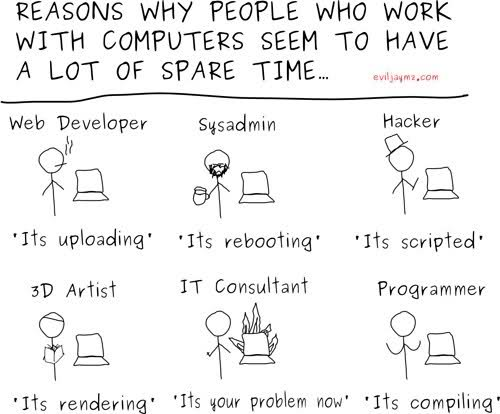
\includegraphics[scale=0.4]{img/sparetime.jpg}
    \end{figure}
\end{frame}

\backupend

\end{document}
